\chapter{Mengen und Abbildungen}
Wir haben bereits im ersten Semester gesehen, wie wichtig Mengen und Abbildungen in
der Informatik sind.  In diesem Kapitel zeigen wir, wie sich Mengen und Abbildungen
effizient implementieren lassen.  Wir k\"onnen  uns auf Abbildungen beschr\"anken, denn eine
Menge $M$ l\"asst sich immer als eine Abbildung $f$ in die Menge $\{\mathtt{true}, \mathtt{false}\}$
darstellen, wenn wir
\\[0.2cm]
\hspace*{1.3cm}
$x \in M \; \Leftrightarrow \; f(x) = \mathtt{true}$
\\[0.2cm]
definieren.  Der Rest dieses Kapitels ist wie folgt aufgebaut:
\begin{enumerate}
\item Zun\"achst definieren wir einen abstrakten Daten-Typ, der Abbildungen spezifiziert.

      Anschlie{\ss}end stellen wir verschiedene Implementierungen dieses Daten-Typs vor.

\item Wir beginnen mit geordneten bin\"aren B\"aumen.
\item Da die Komplexit\"at der Implementierung, die auf geordneten bin\"aren B\"aumen basiert,
      im schlechtesten Fall linear mit der Anzahl der Entr\"age w\"achst, betrachten wir als
      n\"achstes \emph{balancierte bin\"are B\"aume}.  Bei diesen w\"achst die Komplexit\"at der
      Operationen auch im schlechtesten Fall nur logarithmisch mit der Zahl der Eintr\"age.
\item Anschlie{\ss}end betrachten wir die Daten-Struktur der \emph{Tries}, die dann verwendet
      werden kann, wenn die Schl\"ussel, nach denen gesucht werden soll, String sind.
\item \textsl{Hash-Tabellen} stellen eine weitere M\"oglichkeit zur Implementierung
      von Abbildungen dar und werden im vierten Abschnitt diskutiert.
\item Im f\"unften Abschnitt diskutieren wir, welche vordefinierten Datenstrukturen zur
      Implementierung von Abbildungen  dem Entwickler in der Sprache \textsl{Java} zur
      Verf\"ugung gestellt werden.
\item Im letzten Abschnitt zeigen wir als Anwendung, wie das
      \emph{Wolf-Ziege-Kohl}-Problem, das wir bereits im ersten Semester diskutiert
      hatten, in \textsl{Java} gel\"ost werden kann.
\end{enumerate}

\section{Der abstrakte Daten-Typ der \emph{Abbildung}} 
In vielen Anwendungen der Informatik spielen \emph{Abbildungen} einer Menge von
sogenannten \emph{Schl\"usseln} in eine Menge von sogenannten \emph{Werten} eine wichtige
Rolle. Als ein Beispiel betrachten wir ein elektronisches Telefon-Buch wie es
beispielsweise von einem Handy zur Verf\"ugung gestellt wird.  Die wesentlichen
Funktionen, die ein solches Telefon-Buch anbietet, sind:
\begin{enumerate}
\item Nachschlagen eines gegebenen Namens und Ausgabe der diesem Namen zugeordneten
      Telefon-Nummer.
\item Einf\"ugen eines neuen Eintrags mit Namen und Telefon-Nummer.
\item L\"oschen eines vorhandenen Eintrags.
\end{enumerate}
Im Falle des Telefon-Buchs sind die \emph{Schl\"ussel} die Namen und die \emph{Werte} sind
die Telefon-Nummern.  

\begin{Definition}[Abbildung] \hspace*{\fill} \\
{\em
  Wir definieren den abstrakten Daten-Typ der \emph{Abbildung} wie folgt:
  \begin{enumerate}
  \item Als Namen w\"ahlen wir \textsl{Map}.
  \item Die Menge der Typ-Parameter ist $\{ \textsl{Key}, \textsl{Value} \}$.
  \item Die Menge der Funktions-Zeichen ist \\[0.1cm]
       \hspace*{1.3cm} 
       $\{ \textsl{Map}, \textsl{find}, \textsl{insert}, \textsl{delete} \}$.
  \item Die Typ-Spezifikationen der Funktions-Zeichen sind gegeben durch:
        \begin{enumerate}
        \item $\textsl{Map}: \textsl{Map}$

              Der Aufruf $\textsl{Map}()$ erzeugt eine leere Abbildung, also
              eine Abbildung, die keinem Schl\"ussel einen Wert zuweist.
        \item $\textsl{find}: \textsl{Map} \times \textsl{Key} \rightarrow \textsl{Value} \cup \{\Omega\}$

              Der Aufruf $M.\textsl{find}(k)$ \"uberpr\"uft, ob in der Abbildung $M$
              zu dem Schl\"ussel $k$ ein Wert abgespeichert ist.  Wenn ja, wird dieser Wert
              zur\"uck gegeben, sonst wird der Wert $\Omega$ zur\"uck gegeben.
        \item $\textsl{insert}: \textsl{Map} \times \textsl{Key} \times \textsl{Value} \rightarrow \textsl{Map}$

              Der Aufruf $M.\textsl{insert}(k,v)$ f\"ugt in der Abbildung $M$
              f\"ur den Schl\"ussel $k$ den Wert $v$ ein.  Falls zu dem Schl\"ussel $k$ bereits
              ein Eintrag in der Abbildung $M$ existiert, so wird dieser \"uberschrieben.
              Andernfalls wird ein entsprechender Eintrag neu angelegt.
              Als Ergebnis wird die ge\"anderte Abbildung zur\"uck gegeben.
        \item $\textsl{delete}: \textsl{Map} \times \textsl{Key} \rightarrow \textsl{Map}$

              Der Aufruf $M.\textsl{delete}(k)$ entfernt den Eintrag zu dem Schl\"ussel $k$
              in der Abbildung $M$.  Falls kein solcher Eintrag existiert, bleibt die 
              Abbildung $M$ unver\"andert.  Als Ergebnis wird die eventuell ge\"anderte
              Abbildung zur\"uck gegeben.
        \end{enumerate}
  \item Das genaue Verhalten der Funktionen wird durch die nachfolgenden Axiome
        spezifiziert.
        \begin{enumerate}
        \item $\textsl{Map}().\textsl{find}(k) = \Omega$,

              denn der Aufruf $\textsl{Map}()$ erzeugt eine leere Abbildung.
        \item $M.\textsl{insert}(k, v).\textsl{find}(k) = v$,

              denn wenn wir zu dem Schl\"ussel $k$ einen Wert $v$ einf\"ugen, so finden 
              wir anschlie{\ss}end eben diesen Wert $v$, wenn wir nach $k$ suchen.
        \item $k_1 \not= k_2 \rightarrow M.\textsl{insert}(k_1, v).\textsl{find}(k_2) = M.\textsl{find}(k_2)$,

              denn wenn wir f\"ur einen Schl\"ussel eine Wert einf\"ugen, so \"andert das
              nichts an dem Wert, der f\"ur einen anderen Schl\"ussel abgespeichert ist.
        \item $M.\textsl{delete}(k).\textsl{find}(k) = \Omega$,

              denn wenn wir einen Schl\"ussel l\"oschen, so finden wir anschlie{\ss}end auch
              keinen Wert mehr unter diesem Schl\"ussel.
        \item $k_1 \not= k_2 \rightarrow M.\textsl{delete}(k_1).\textsl{find}(k_2) = M.\textsl{find}(k_2)$,

              denn wenn wir einen Schl\"ussel  l\"oschen, so \"andert das nichts an dem
              Wert, der unter einem anderen Schl\"usseln abgespeichert ist. \hspace*{\fill} $\Box$
        \end{enumerate}
  \end{enumerate}
}
\end{Definition}

%Es ist in \textsc{Setl2} sehr einfach, den ADT \textsl{Abbildung} zu implementieren.
%Dazu m\"ussen wir uns nur klar machen, dass Abbildungen nichts anderes sind als Funktionen
%und die k\"onnen wir in der Mengenlehre durch bin\"are Relationen darstellen.
%Ist $R$ eine bin\"are Relation die genau ein Paar der Form $[k,v]$ enth\"alt, so liefert der Ausdruck \\[0.1cm]
%\hspace*{1.3cm} $R(k)$
%\\[0.1cm]
%als Ergebnis den Wert $v$.  Umgekehrt wird durch den Aufruf \\[0.1cm]
%\hspace*{1.3cm} $R(k) := v$ \\[0.1cm]
%das Paar $[k,v]$ in die Relation $R$ eingef\"ugt.  Um den Eintrag unter einem Schl\"ussel $k$
%zu l\"oschen, reicht es aus, dem Schl\"ussel $k$ den undefinierten Wert $\Omega$ zuzuweisen: \\[0.1cm]
%\hspace*{1.3cm} $R(k) := \Omega$. \\[0.1cm]
%Dieser Wert wird auch bei der Auswertung des Ausdrucks $R(k)$ zur\"uck gegeben, wenn die
%bin\"are Relation kein Paar der Form $[k,v]$ enth\"alt.

%Abbildung \ref{fig:map-trivial} zeigt
%eine Implementierung des ADT Abbildung, die auf diesen Überlegungen aufbaut.

%\begin{figure}[!ht]
%  \centering
%\begin{Verbatim}[ frame         = lines, 
%                  framesep      = 0.3cm, 
%                  labelposition = bottomline,
%                  numbers       = left,
%                  numbersep     = -0.2cm,
%                  xleftmargin   = 0.8cm,
%                  xrightmargin  = 0.8cm
%                ]
%    class Map;    
%        procedure create(); -- implementiert Konstruktor Map
%        procedure find(k);
%        procedure insert(k, v);
%        procedure delete(k);
%    end Map;
    
%    class body Map;
    
%        var relation;
%        -- Konstruktor   
%        procedure create();
%            relation := {};
%        end create;
    
%        procedure find(k);
%            return relation(k);
%        end find;
    
%        procedure insert(k, v);
%            relation(k) := v;
%        end insert;
    
%        procedure delete(k);
%            relation(k) := om;
%        end delete;
        
%    end Map;
%\end{Verbatim}
%\vspace*{-0.3cm}
%  \caption{Eine triviale Implementierung des ADT \textsl{Map}}
%  \label{fig:map-trivial}
%\end{figure} 


\section{Geordnete bin\"are B\"aume}
Falls auf der Menge \textsl{Key} der Schl\"ussel eine totale Ordnung $\leq$ existiert, so kann
eine einfache und zumindest im statistischen Durchschnitt effiziente Implementierung des
abstrakte Daten-Typs \textsl{Map} mit Hilfe \emph{geordneter bin\"arer B\"aume} erfolgen.
Um diesen Begriff definieren zu k\"onnen, f\"uhren wir zun\"achst \emph{bin\"are B\"aume} ein.

\begin{Definition}[Bin\"arer Baum] \hspace*{\fill} \\
{\em
  Gegeben sei eine Menge $\textsl{Key}$ von Schl\"usseln und eine Menge $\textsl{Value}$ von
  Werten.  Dann definieren wir
  die Menge der bin\"aren B\"aume $\Bin$ induktiv mit Hilfe der
  beiden Funktions-Zeichen \textsl{nil} und \textsl{node}, deren Typ-Spezifikationen 
  wie folgt gegeben sind: \\[0.1cm]
  \hspace*{1.3cm} 
  $\textsl{nil}: \Bin$ \qquad und \qquad  $\textsl{node}: \textsl{Key} \times \textsl{Value} \times \Bin \times \Bin \rightarrow \Bin$.
  \begin{enumerate}
  \item $\textsl{nil}$ ist ein bin\"arer Baum.

        Dieser Baum wird als der \emph{leere Baum} bezeichnet.
  \item $\textsl{node}(k, v, l, r)$ ist ein bin\"arer Baum, falls gilt: 
        \begin{enumerate}
        \item $k$ ist ein Schl\"ussel aus der Menge $\textsl{Key}$.
        \item $v$ ist ein Wert aus der Menge $\textsl{Value}$.
        \item $l$ ist ein bin\"arer Baum.

              $l$ wird als der \emph{linke Teilbaum} von $\textsl{node}(k, v, l, r)$ bezeichnet.
        \item $r$ ist ein bin\"arer Baum.

              $r$ wird als der \emph{rechte Teilbaum} von $\textsl{node}(k, v, l, r)$ bezeichnet.
              \hspace*{\fill} $\Box$
        \end{enumerate}
  \end{enumerate}
}
\end{Definition}

\noindent
Als n\"achstes definieren wir, was wir unter einem \emph{geordneten bin\"aren Baum} verstehen.
\begin{Definition}[Geordneter bin\"arer Baum] \hspace*{\fill} \\
{\em
  Die Menge $\Bin_<$ der \emph{geordneten bin\"aren B\"aume} wird induktiv definiert.
  \begin{enumerate}
  \item $\textsl{nil} \in \Bin_<$
  \item $\textsl{node}(k, v, l, r) \in \Bin_<$ \quad falls folgendes gilt:
        \begin{enumerate}
        \item $k$ ist ein Schl\"ussel aus der Menge $\textsl{Key}$.
        \item $v$ ist ein Wert aus der Menge $\textsl{Value}$.
        \item $l$ und $r$ sind geordnete bin\"are B\"aume.
        \item Alle Schl\"ussel, die in dem linken Teilbaum $l$ auftreten,
              sind kleiner als $k$.
        \item Alle Schl\"ussel, die in dem rechten Teilbaum $r$ auftreten,
              sind gr\"o{\ss}er als $k$.
        \end{enumerate}
        Die beiden letzten  Bedingungen bezeichnen wir als die \emph{Ordnungs-Bedingung}.
        \hspace*{\fill} $\Box$
  \end{enumerate}
}  
\end{Definition}
Geordnete bin\"are B\"aume lassen sich grafisch wir folgt darstellen:
\begin{enumerate}
\item Der leere Baum \textsl{nil} wird durch einen dicken schwarzen Punkt dargestellt.
\item Ein Baum der Form $\textsl{node}(k,v,l,r)$ wird dargestellt,  indem zun\"achst ein
      Oval gezeichnet wird, in dem oben der Schl\"ussel $k$ und darunter, getrennt durch
      einen waagerechten Strich, der dem Schl\"ussel zugeordnete Wert $v$ eingetragen wird.
      Dieses Oval bezeichnen wir auch als einen \emph{Knoten} des bin\"aren Baums.
      Anschlie{\ss}end wird links unten von diesem Knoten rekursiv der Baum $l$ gezeichnet
      und  rechts unten wird rekursiv der Baum $r$ gezeichnet. Zum Abschluss zeichnen wir
      von dem mit $k$ und $v$ markierten Knoten jeweils einen Pfeil zu dem linken und dem
      rechten Teilbaum.
\end{enumerate}
Abbildung \ref{fig:graph1} zeigt ein Beispiel f\"ur einen
geordneten bin\"aren Baum.  Der oberste Knoten, in der Abbildung ist das der mit dem Schl\"ussel
$8$ und dem Wert $22$ markierte Knoten, wird als die \emph{Wurzel} des Baums bezeichnet.
Ein \emph{Pfad der L\"ange} $k$ in dem Baum ist eine Liste $[n_0,n_1, \cdots, n_k]$ von
$k+1$ Knoten, die durch Pfeile verbunden sind. Identifizieren wir Knoten mit ihren
Markierungen, so ist \\[0.1cm]
\hspace*{1.3cm} $\bigl[ \pair(8,22), \pair(12,18), \pair(10,16), \pair(9,39) \bigr]$ \\[0.1cm]
ein Pfad der L\"ange 3.


\begin{figure}[!ht]
  \centering
  \framebox{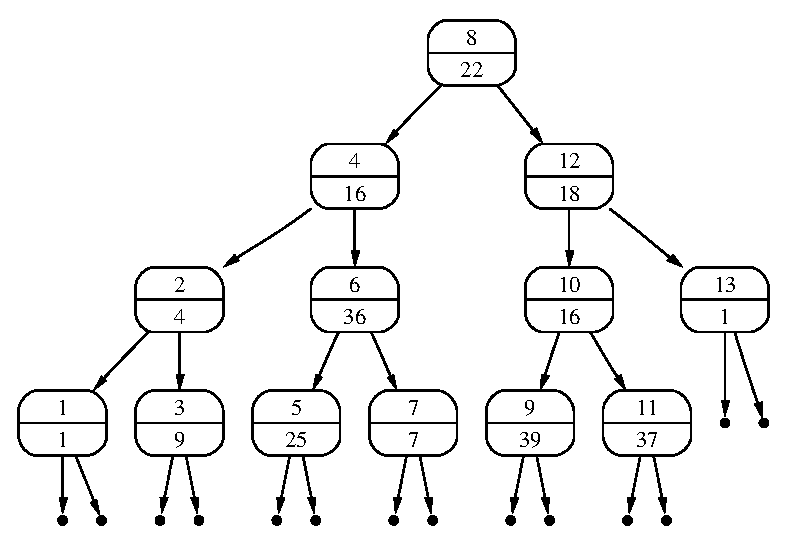
\epsfig{file=Abbildungen/graph1.eps}} 
  \caption{Ein geordneter bin\"arer Baum}
  \label{fig:graph1}
\end{figure}


Wir \"uberlegen uns nun, wie wir mit Hilfe geordneter bin\"arer B\"aume den ADT \textsl{Map}
implementieren k\"onnen.  Wir spezifizieren die einzelnen Methoden dieses Daten-Typs durch
(bedingte) Gleichungen.  Der Konstruktor $\textsl{Map}()$ liefert als Ergebnis den leeren Baum zur\"uck:
\[ \textsl{Map}() = \textsl{nil}. \]
F\"ur die Methode $\textsl{find}()$ erhalten wir die folgenden Gleichungen:
\begin{enumerate}
\item $\textsl{nil}\mathtt{.}\textsl{find}(k) = \Omega$,

      denn der leere Baum repr\"asentiert die leere Abbildung.
\item $\textsl{node}(k, v, l, r)\mathtt{.}\textsl{find}(k) = v$,

      denn der Knoten $\textsl{node}(k,v,l,r)$ speichert die Zuordnung $k \mapsto v$.
\item $k_1 < k_2 \rightarrow \textsl{node}(k_2, v, l, r)\mathtt{.}\textsl{find}( k_1) = l\mathtt{.}\textsl{find}(k_1)$,

      denn wenn $k_1$ kleiner als $k_2$ ist, dann kann aufgrund der Ordnungs-Bedingung
      eine Zuordnung f\"ur $k_1$ nur in dem linken Teilbaum $l$ gespeichert sein.
\item $k_1 > k_2 \rightarrow \textsl{node}(k_2, v, l, r)\mathtt{.}\textsl{find}( k_1 ) = r\mathtt{.}\textsl{find}(k_1)$,

      denn wenn $k_1$ gr\"o{\ss}er als $k_2$ ist, dann kann aufgrund der Ordnungs-Bedingung
      eine Zuordnung f\"ur $k_1$ nur in dem rechten Teilbaum $r$ gespeichert sein.
\end{enumerate}
Als n\"achstes definieren wir die Funktion \textsl{insert}.  Die Definition erfolgt
ebenfalls mit Hilfe rekursiver Gleichungen und ist ganz analog zur Definition der 
Funktion \textsl{find}.
\begin{enumerate}
\item $\textsl{nil}\mathtt{.}\textsl{insert}(k,v) = \textsl{node}(k,v, \textsl{nil}, \textsl{nil})$,
  
      denn wenn der Baum vorher leer ist, so kann die einzuf\"ugende Information direkt an
      der Wurzel abgespeichert werden.
\item $\textsl{node}(k, v_2, l, r)\mathtt{.}\textsl{insert}(k,v_1) = \textsl{node}(k, v_1, l, r)$,

      denn wenn wir den Schl\"ussel $k$ an der Wurzel finden, \"uberschreiben wir einfach den zugeordneten 
      Wert.
\item $k_1 < k_2 \rightarrow 
          \textsl{node}(k_2, v_2, l, r)\mathtt{.}\textsl{insert}(k_1, v_1) =
          \textsl{node}\bigl(k_2, v_2, l\mathtt{.}\textsl{insert}(k_1, v_1), r\bigr)$,

      denn wenn der Schl\"ussel $k_1$, unter dem wir Informationen einf\"ugen wollen, kleiner
      als der Schl\"ussel $k_2$ an der Wurzel ist, so m\"ussen wir die einzuf\"ugende
      Information im linken Teilbaum einf\"ugen.
\item $k_1 > k_2 \rightarrow 
         \textsl{node}(k_2, v_2, l, r)\mathtt{.}\textsl{insert}(k_1, v_1) = 
         \textsl{node}\bigl(k_2, v_2, l, r\mathtt{.}\textsl{insert}(k_1, v_1)\bigr)$,

      denn wenn der Schl\"ussel $k_1$, unter dem wir Informationen einf\"ugen wollen, gr\"o{\ss}er
      als der Schl\"ussel $k_2$ an der Wurzel ist, so m\"ussen wir die einzuf\"ugende
      Information im rechten Teilbaum einf\"ugen.
\end{enumerate}
Als letztes definieren wir die Methode \textsl{delete}. Diese Definition ist schwieriger als
die Implementierung der andern beiden Methoden.  Falls wir in einen Baum der Form
$t =\textsl{node}(k,v,l,r)$ den Eintrag mit dem Schl\"ussel $k$ l\"oschen wollen, so
kommt es auf die beiden Teilb\"aume $l$ und $r$ an.  Ist $l$ der leere Teilbaum,
so liefert $t\mathtt{.}\textsl{delete}(k)$ als Ergebnis den Teilbaum $r$ zur\"uck.
Ist $r$ der leere Teilbaum, so ist das Ergebnis $l$.  Problematisch ist die Situation,
wenn weder $l$ noch $r$ leer sind.  
Die L\"osung besteht dann darin, dass wir in dem rechten
Teilbaum $r$ den Knoten mit dem kleinsten Schl\"ussel suchen und diesen Knoten aus dem
Baum $r$ entfernen.  Den dadurch entstehenden Baum nennen wir $r'$.
 Anschlie{\ss}end \"uberschreiben wir in $t =\textsl{node}(k,v,l,r')$ die
Werte $k$ und $v$ mit dem eben gefundenen kleinsten Schl\"ussel $k_{min}$ und dem $k_{min}$
zugeordneten Wert $v_{min}$.  Der dadurch entstehende bin\"are Baum 
$t=\textsl{node}(k_{min},v_{min},l,r')$
 ist auch wieder
geordnet, denn einerseits ist der Schl\"ussel $k_{min}$  gr\"o{\ss}er als der Schl\"ussel $k$ und
damit sicher auch gr\"o{\ss}er als alle Schl\"ussel im linken Teilbaum $l$ und andererseits ist
$k_{min}$ kleiner als alle  Schl\"ussel im Teilbaum $r'$ den $k_{min}$ ist ja der
kleinste Schl\"ussel aus $r$.  

Zur Veranschaulichung betrachten wir ein Beispiel: Wenn wir in dem Baum aus Abbildung 
\ref{fig:graph1} den Knoten mit der Markierung $\pair(4,16)$ l\"oschen wollen,
so suchen wir zun\"achst in dem Teilbaum, dessen Wurzel mit $\pair(6,36)$ markiert ist, den
Knoten, der mit dem kleinsten Schl\"ussel markiert ist.  Dies ist der Knoten mit der
Markierung $\pair(5,25)$.  Wir l\"oschen diesen Knoten und \"uberschreiben die Markierung
$\pair(4,16)$ mit der Markierung $\pair(5,25)$.  Abbildung 
\ref{fig:graph2} auf Seite \pageref{fig:graph2} zeigt das Ergebnis.

\begin{figure}[!th]
  \centering
  \framebox{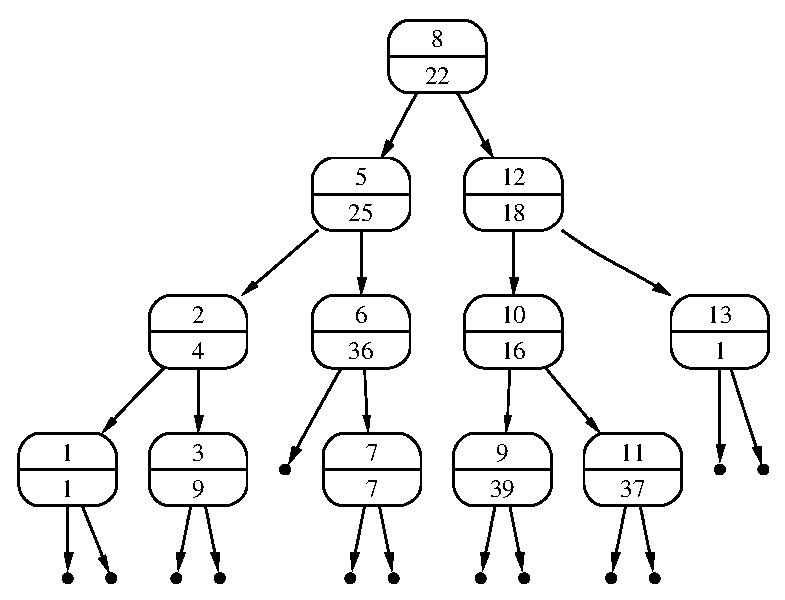
\epsfig{file=graph2.eps}} 
  \caption{Der geordnete bin\"arer Baum aus Abbildung 
          \ref{fig:graph1} nach dem Entfernen des Knotens mit der Markierung $\pair(4,16)$.}
  \label{fig:graph2}
\end{figure}

Wir geben nun bedingte Gleichungen an, die die Methode \textsl{delMin} spezifizieren.
\begin{enumerate}
\item $\textsl{node}(k, v, \textsl{nil}, r)\mathtt{.}\textsl{delMin}() = [r, k, v]$,

      denn wenn der linke Teilbaum leer ist, muss $k$ der kleinste Schl\"ussel in 
      dem Baum sein.  Wenn wir diesen  Schl\"ussel nebst dem zugeh\"origen Wert aus dem Baum
      entfernen, bleibt der rechte Teilbaum \"ubrig.

\item $l\not= \textsl{nil} \wedge l\mathtt{.}\textsl{delMin}() = [l',k_{min}, v_{min}] \;\rightarrow$ \\[0.1cm]
       \hspace*{1.3cm} 
       $\textsl{node}(k, v, l, r)\mathtt{.}\textsl{delMin}() = [\textsl{node}(k, v, l', r), k_{min}, v_{min}]$,

      denn wenn der linke Teilbaum $l$ in dem bin\"aren Baum $t = \textsl{node}(k, v, l, r)$
      nicht leer ist, so muss der kleinste Schl\"ussel von $t$ in $l$ liegen.
      Wir entfernen daher rekursiv den kleinsten Schl\"ussel aus $l$ und erhalten dabei den
      Baum $l'$.  In dem urspr\"unglich gegebenen Baum $t$ ersetzen wir $l$ durch $l'$ und erhalten
      $t = \textsl{node}(k, v, l', r)$.
\end{enumerate}
Damit k\"onnen wir nun die Methode $\mathtt{delete}()$ spezifizieren.
\begin{enumerate}
\item $\textsl{nil}\mathtt{.}\textsl{delete}(k) = \textsl{nil}$.
\item $\textsl{node}(k,v,\textsl{nil},r)\mathtt{.}\textsl{delete}(k) = r$.
\item $\textsl{node}(k,v,l,\textsl{nil})\mathtt{.}\textsl{delete}(k) = l$.
\item $l \not= \textsl{nil} \,\wedge\, r \not= \textsl{nil} \,\wedge\, r\mathtt{.}\textsl{delMin}() = [r',k_{min}, v_{min}]  \;\rightarrow$ \\[0.1cm]
      \hspace*{1.3cm}
      $\textsl{node}(k,v,l,r)\mathtt{.}\textsl{delete}(k) = \textsl{node}(k_{min},v_{min},l,r')$.
      
      Falls der zu entfernende Schl\"ussel mit dem Schl\"ussel an der Wurzel des Baums
      \"ubereinstimmt,  entfernen wir mit dem Aufruf $r\mathtt{.}\textsl{delMin}()$
      den kleinsten Schl\"ussel aus dem rechten Teilbaum  $r$ und produzieren dabei den Baum $r'$.
      Gleichzeitig berechnen wir dabei f\"ur den rechten Teilbaum den kleinsten Schl\"ussel $k_{min}$ und den
      diesem Schl\"ussel zugeordneten Wert $v_{min}$.  Diese Werte setzen wir nun an die
      Wurzel des neuen Baums.

\item $k_1 < k_2 \rightarrow \textsl{node}(k_2,v_2,l,r)\mathtt{.}\textsl{delete}(k_1) = 
       \textsl{node}\bigl(k_2,v_2,l\mathtt{.}\textsl{delete}(k_1),r\bigr)$,

      Falls der zu entfernende Schl\"ussel kleiner ist als der Schl\"ussel an der Wurzel,
      so kann sich der Schl\"ussel nur im linken Teilbaum befinden.  Daher wird der
      Schl\"ussel $k_1$ rekursiv in dem linken Teilbaum $l$ entfernt.
\item $k_1 > k_2 \rightarrow \textsl{node}(k_2,v_2,l,r)\mathtt{.}\textsl{delete}(k_1) = 
       \textsl{node}\bigl(k_2,v_2,l,r\mathtt{.}\textsl{delete}(k_1)\bigr)$,

      denn in diesem Fall kann sich der Eintrag mit dem Schl\"ussel $k_1$  nur im rechten Teilbaum befinden.
\end{enumerate}

\subsection{Implementierung geordneter bin\"arer B\"aume in \textsl{Java}}
\begin{figure}[!ht]
  \centering
\begin{Verbatim}[ frame         = lines, 
                  framesep      = 0.3cm, 
                  labelposition = bottomline,
                  numbers       = left,
                  numbersep     = -0.2cm,
                  xleftmargin   = 0.8cm,
                  xrightmargin  = 0.8cm
                ]
    public interface MyMap<Key extends Comparable<Key>, Value>
    {
        public Value find(Key key);
        public void  insert(Key key, Value value);
        public void  delete(Key key);
    }
\end{Verbatim}
\vspace*{-0.3cm}
  \caption{Das Interface  \textsl{MyMap}.}
  \label{fig:MyMap.java}
\end{figure}

Abbildung \ref{fig:MyMap.java} auf Seite \pageref{fig:MyMap.java} zeigt, 
wie sich der abstrakte Daten-Typ \textsl{Map} in \textsl{Java} durch ein
Interface beschreiben l\"asst.  Das Interface hat den Namen \textsl{MyMap}, denn da der ADT
\textsl{Map} von  fundamentaler Bedeutung ist, gibt es in \textsl{Java} bereits ein
Interface mit dem Namen \textsl{Map}.  Vergleichen wir die Signaturen der Methoden in dem
Interface \textsl{MyMap} mit den entsprechenden Signaturen in dem ADT \textsl{Map}, so
stellen wir fest, dass die Methoden \texttt{insert()} und \texttt{delete()} in dem
Interface den R\"uckgabewert \texttt{void} an Stelle von \textsl{MyMap} haben.
Anstatt also eine ge\"anderte Map zur\"uck zu geben \"andern diese Methoden die Map, mit der sie
aufgerufen werden.  Dies ist einerseits aus Effizienz-Gr\"unden wichtig und macht
andererseits die Verwendung dieser Methoden einfacher.


\begin{figure}[!ht]
  \centering
\begin{Verbatim}[ frame         = lines, 
                  framesep      = 0.3cm, 
                  labelposition = bottomline,
                  numbers       = left,
                  numbersep     = -0.2cm,
                  xleftmargin   = 0.8cm,
                  xrightmargin  = 0.8cm
                ]
    public class BinaryTree<Key extends Comparable<Key>, Value> 
        implements MyMap<Key, Value>
    {
        Node<Key, Value> mRoot;  
    
        public BinaryTree() {
            mRoot = new EmptyNode<Key, Value>();
        }
        public Value find(Key key) {
            return mRoot.find(key);
        }    
        public void insert(Key key, Value value) {
            mRoot = mRoot.insert(key, value);
        }
        public void delete(Key key) {
            mRoot = mRoot.delete(key);
        }
        // Transform the tree into a sorted list.
        public  LinkedList<Key> toList() {
            return mRoot.toList();
        }
    }
\end{Verbatim}
\vspace*{-0.3cm}
  \caption{Die Klasse \textsl{BinaryTree}.}
  \label{fig:BinTree.java}
\end{figure}



\begin{figure}[!ht]
  \centering
\begin{Verbatim}[ frame         = lines, 
                  framesep      = 0.3cm, 
                  labelposition = bottomline,
                  numbers       = left,
                  numbersep     = -0.2cm,
                  xleftmargin   = 0.8cm,
                  xrightmargin  = 0.8cm
                ]
    public abstract class Node<Key extends Comparable<Key>, Value>
    {
        public abstract Value find(Key key);
        public abstract Node<Key, Value> insert(Key key, Value value);
        public abstract Node<Key, Value> delete(Key key);
        public abstract boolean isEmpty();
        public abstract LinkedList<Key> toList();
    
        abstract Triple<Node<Key, Value>, Key, Value> delMin();
    }
\end{Verbatim}
\vspace*{-0.3cm}
  \caption{Die abstrakte Klasse \textsl{Node}.}
  \label{fig:Node.java}
\end{figure}

\begin{figure}[!ht]
  \centering
\begin{Verbatim}[ frame         = lines, 
                  framesep      = 0.3cm, 
                  labelposition = bottomline,
                  numbers       = left,
                  numbersep     = -0.2cm,
                  xleftmargin   = 0.8cm,
                  xrightmargin  = 0.8cm
                ]
    public class EmptyNode<Key extends Comparable<Key>, Value> 
        extends Node<Key, Value>
    {
        public EmptyNode() {}
        
        public Value find(Key key) {
            return null;
        }        
        public Node<Key, Value> insert(Key key, Value value) {
            return new BinaryNode<Key, Value>(key, value);
        }        
        public Node<Key, Value> delete(Key key) {
            return this;
        }
        public boolean isEmpty() {
            return true;
        }    
        public LinkedList<Key> toList() {
            return new LinkedList<Key>();
        }
        Triple<Node<Key, Value>, Key, Value> delMin() {
            throw new UnsupportedOperationException();
        }
    }
\end{Verbatim}
\vspace*{-0.3cm}
  \caption{Die Klasse \textsl{EmptyNode}.}
  \label{fig:EmptyNode.java}
\end{figure}

Abbildung \ref{fig:BinTree.java} auf Seite \pageref{fig:BinTree.java} zeigt die 
Implementierung der Klasse \textsl{BinTree} in \textsl{Java}.  Die Klasse enth\"alt ein
Objekt vom Typ \textsl{Node} mit dem Namen \texttt{mRoot}.  Dieser Knoten repr\"asentiert
die Wurzel des bin\"aren Baums.  Die Methoden der Klasse \textsl{BinTree} werden dadurch
implementiert, dass die analogen Methoden der abstrakten Klasse \textsl{Node} aufgerufen
werden.  
Abbildung \ref{fig:Node.java} auf Seite \pageref{fig:Node.java} zeigt die Definition
der Klasse \textsl{Node}.  Bei der Betrachtung der Signaturen der Methoden stellen wir
fest, dass die Methoden \textsl{insert()} und \textsl{delete()} nun einen R\"uckgabewert
haben.   Dies ist n\"otig, weil in \textsl{Java} ein Objekt seinen Typ nicht \"andern kann.  
Von der Klasse \textsl{Node} werden zwei konkrete Klassen abgeleitet:  Die Klasse
\textsl{EmptyNode} repr\"asentiert einen leeren bin\"aren Baum, entspricht also dem
\textsl{nil} und die Klasse \textsl{BinaryNode} dient dazu, einen Knoten der Form
$\textsl{node}(k,v,l,r)$ darzustellen.  Nun ist es so, dass beim Einf\"ugen  aus
einem leeren Baum ein nicht-leerer Baum werden kann und umgekehrt kann beim L\"oschen 
aus einem nicht-leeren Baum ein leerer Baum werden.  Da aber die Methode \textsl{insert()}
ein Objekt vom Typ \textsl{EmptyNode} nicht in ein Objekt \textsl{BinaryNode} umwandeln
kann, muss die Methoden \textsl{insert()} statt dessen den bin\"aren Baum, der durch das
Einf\"ugen eines Schl\"ussels entsteht, als  Ergebnis zur\"uck geben.  Analoges gilt f\"ur die
Methode \textsl{delete()}.

\begin{figure}[!ht]
  \centering
\begin{Verbatim}[ frame         = lines, 
                  framesep      = 0.3cm, 
                  labelposition = bottomline,
                  numbers       = left,
                  numbersep     = -0.2cm,
                  xleftmargin   = 0.0cm,
                  xrightmargin  = 0.0cm
                ]
    public class BinaryNode<Key extends Comparable<Key>, Value> 
        extends Node<Key, Value>
    {
        private Key              mKey;     /**< The key stored at the root. */
        private Value            mValue;   /**< The value attached to this key. */
        private Node<Key, Value> mLeft;    /**< The left subtree. */
        private Node<Key, Value> mRight;   /**< The right subtree. */
    
        public BinaryNode(Key key, Value value) {
            mKey   = key;
            mValue = value;
            mLeft  = new EmptyNode<Key, Value>();
            mRight = new EmptyNode<Key, Value>();
        }        
        public Value find(Key key) {
            int cmp = key.compareTo(mKey);
            if (cmp < 0) {                // key < mKey
                return mLeft.find(key);
            } else if (cmp > 0) {         // key > mKey
                return mRight.find(key);
            } else {                      // key == mKey
                return mValue;
            }            
        }
        public Node<Key, Value> insert(Key key, Value value) {
            int cmp = key.compareTo(mKey);
            if (cmp < 0) {                        // key < mKey
                mLeft = mLeft.insert(key, value);
            } else if (cmp > 0) {                 // key > mKey
                mRight = mRight.insert(key, value);
            } else {                              // key == mKey
                mValue = value;
            }            
            return this;
        }
\end{Verbatim}
\vspace*{-0.3cm}
  \caption{Die Klasse \textsl{BinaryNode}, Teil \texttt{I}.}
  \label{fig:BinaryNode-I.java}
\end{figure}

\begin{figure}[!ht]
  \centering
\begin{Verbatim}[ frame         = lines, 
                  framesep      = 0.3cm, 
                  firstnumber   = last,
                  labelposition = bottomline,
                  numbers       = left,
                  numbersep     = -0.2cm,
                  xleftmargin   = 0.0cm,
                  xrightmargin  = 0.0cm
                ]
        public Node<Key, Value> delete(Key key) {
            int cmp = key.compareTo(mKey);
            if (cmp == 0) {
                if (mLeft.isEmpty()) {
                    return mRight;
                } 
                if (mRight.isEmpty()) {
                    return mLeft;
                }
                Triple triple = mRight.delMin();
                mRight = triple.getFirst();
                mKey   = triple.getSecond();
                mValue = triple.getThird();
            }
            if (cmp < 0) {
                mLeft = mLeft.delete(key);
            }
            if (cmp > 0) {
                mRight = mRight.delete(key);
            }
            return this;
        }    
        public boolean isEmpty() {
            return false;
        }
        Triple delMin() {
            if (mLeft.isEmpty()) {
                return new Triple<Node<Key, Value>, Key, Value>(mRight, mKey, mValue);
            } else {
                Triple<Node<Key, Value>, Key, Value> t = mLeft.delMin();
                      mLeft = t.getFirst();
                Key   key   = t.getSecond();
                Value value = t.getThird();
                return new Triple<Node<Key, Value>, Key, Value>(this, key, value);
            }
        }        
    }
\end{Verbatim}
\vspace*{-0.3cm}
  \caption{Die Klasse \textsl{BinaryNode}, Teil \texttt{II}.}
  \label{fig:BinaryNode-II.java}
\end{figure}
\vspace*{0.1cm}

Gegen\"uber den Methoden aus der Klasse \textsl{BinaryTree} hat die Klasse \textsl{Node} die
zus\"atzliche Methode \textsl{isEmpty()} die \"uberpr\"uft, ob der Knoten den leeren Baum
repr\"asentiert. Au{\ss}erdem gibt es noch die Methode \textsl{delMin()}, die den Knoten mit dem
kleinsten Schl\"ussel aus einem Baum l\"oscht.  Diese Methode ist nicht als \texttt{public}
deklariert, da sie nur zur Implementierung der Methode \textsl{delete()} benutzt wird.


Abbildung \ref{fig:EmptyNode.java} zeigt die Definition der Klasse \textsl{EmptyNode}.
Bemerkenswert ist hier die Implementierung der Methode \textsl{delMin()}: Da der leere
Baum keine Schl\"ussel enth\"alt, macht die Methode \textsl{delMin()} keinen Sinn.  Daher
produziert der Aufruf dieser Methode eine Ausnahme.


Algorithmisch interessant ist die Implementierung der Klasse \textsl{BinaryNode}, die in den
Abbildungen \ref{fig:BinaryNode-I.java} und \ref{fig:BinaryNode-II.java} auf den Seiten 
\pageref{fig:BinaryNode-I.java} und \pageref{fig:BinaryNode-II.java} gezeigt wird.
Die Klasse enth\"alt vier Member-Variablen:
\begin{enumerate}
\item \texttt{mKey} ist der Schl\"ussel, der an diesem Knoten abgespeichert wird.
\item \texttt{mValue} ist der dem Schl\"ussel \textrm{mKey} zugeordnete Wert.
\item \texttt{mLeft} ist der linke Teilbaum.
\item \texttt{mRight} ist der rechte Teilbaum.
\end{enumerate}
Ein Objekt $o$ der Klasse \textsl{BinaryNode} entspricht also dem Term \\[0.1cm]
\hspace*{1.3cm} 
$\textsl{node}(o.\texttt{mKey}, o.\texttt{mValue}, o.\texttt{mLeft}, o.\texttt{mRight})$. 
\\[0.1cm]
Die Implementierung der Methoden \textsl{find()}, \textsl{insert()} und \textsl{delete()} setzt die bedingten
Gleichungen, mit denen wir diese Methoden spezifiziert haben, eins-zu-eins um.

\begin{figure}[!ht]
  \centering
\begin{Verbatim}[ frame         = lines, 
                  framesep      = 0.3cm, 
                  firstnumber   = last,
                  labelposition = bottomline,
                  numbers       = left,
                  numbersep     = -0.2cm,
                  xleftmargin   = 0.8cm,
                  xrightmargin  = 0.8cm
                ]
    public class Triple<First, Second, Third>
    {
        First  mFirst;
        Second mSecond;
        Third  mThird;
        
        Triple(First first, Second second, Third value) {
            mFirst  = first;
            mSecond = second;
            mThird  = value;
        }
    
        First  getFirst()  { return mFirst;  }
        Second getSecond() { return mSecond; }
        Third  getThird()  { return mThird;  }
    }
\end{Verbatim}
\vspace*{-0.3cm}
  \caption{Die Klasse \textsl{Triple}.}
  \label{fig:Triple.java}
\end{figure}

\noindent
Abbildung \ref{fig:Triple.java} auf Seite \pageref{fig:Triple.java} zeigt schlie{\ss}lich die
Implementierung der Klasse \textsl{Triple}.  Diese Klasse dient dazu ein Tripel
darzustellen und hat folglich drei Member-Variablen \texttt{mFirst}, \texttt{mSecond},
\texttt{mThird}, die jeweils die erste, zweite und dritte Komponente des Tripels abspeichern.
\pagebreak



\subsection{Analyse der Komplexit\"at}
Wir untersuchen zun\"achst die Komplexit\"at der Funktion \textsl{find} im schlechtesten Fall.
Dieser Fall tritt dann ein, wenn der bin\"are Baum zu einer Liste entartet.  Abbildung
\ref{fig:degenerated} zeigt den geordneten bin\"aren Baum der dann entsteht, wenn die Paare
aus Schl\"ussel und Werten aus der Abbildung
\ref{fig:graph1} in aufsteigender Reihenfolge eingegeben werden.  Wird hier nach dem
gr\"o{\ss}ten Schl\"ussel gesucht, so muss der komplette Baum durchlaufen werden.  Enth\"alt der Baum
$n$ Schl\"ussel, so sind also insgesamt $n$ Vergleiche erforderlich.  In diesem Fall ist ein
geordneter bin\"arer Baum also nicht besser als eine Liste.

\begin{figure}[!th]
  \centering
  \framebox{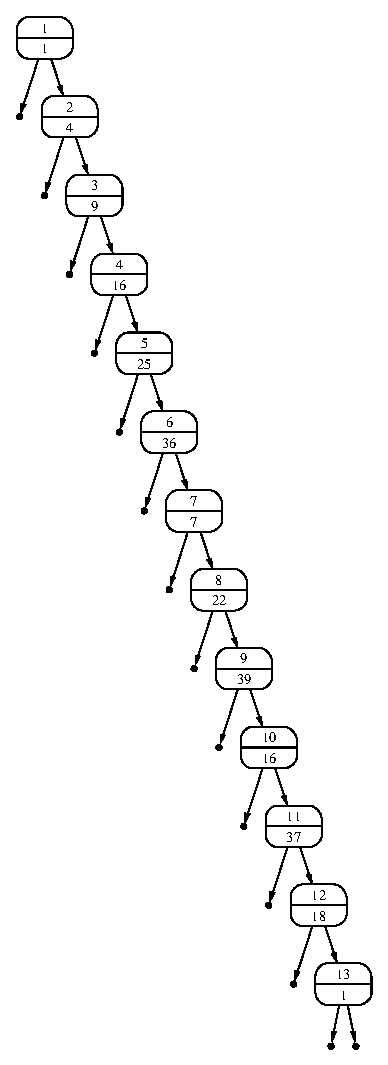
\epsfig{file=degenerated-bin-tree}} 
  \caption{Ein entarteter  geordneter bin\"arer Baum.}
  \label{fig:degenerated}
\end{figure}

Erfreulicherweise tritt der schlechteste Fall im statistischen Durchschnitt selten auf.
Im Durchschnitt ist ein zuf\"allig erzeugter bin\"arer Baum recht gut balanciert, so dass 
beispielsweise f\"ur einen Aufruf von \texttt{find()} f\"ur einen Baum mit $n$ Schl\"usseln
durchschnittlich  $\Oh\bigl(\ln(n)\bigr)$
Vergleiche erforderlich sind. Wir werden diese Behauptung nun beweisen.

%Dazu definieren wir auf bin\"aren B\"aumen zun\"achst eine Funktion 
%\[ \textsl{height}: \Bin \rightarrow \N, \]
%die die H\"ohe eines bin\"aren Baums angibt.  Die Definition erfolgt induktiv.
%\begin{enumerate}
%\item $\textsl{nil}.\textsl{height}() = 0$.

%      Der leere Baum hat die H\"ohe $0$.
%\item $\textsl{node}(k,v,l,r).\textsl{height}() = 
%       1 + \max\bigl(l.\textsl{height}(),\, r.\textsl{height}()\bigr)$.

%      Die H\"ohe des Baums $\textsl{node}(k,v,l,r)$ ist um eins gr\"o{\ss}er als die H\"ohe des
%      gr\"o{\ss}ten Teilbaums.
%\end{enumerate}
%Analog definieren wir f\"ur einen bin\"aren Baum $b$ die Anzahl $b.\textsl{count}()$ der Schl\"ussel, die
%der Baum enth\"alt.   Die Definition von $b.\textsl{count}()$ erfolgt durch Induktion nach $b$.
%\begin{enumerate}
%\item $\textsl{nil}.\textsl{count}() = 0$.

%      Der leere Baum enth\"alt keine Schl\"ussel.
%\item $\textsl{node}(k,v,l,r).\textsl{count}() = 
%       1 + l.\textsl{count}() + r.\textsl{height}()\bigr)$.

%      Der Baum $\textsl{node}(k,v,l,r)$ enth\"alt zus\"atzlich zu dem Schl\"ussel $k$ die
%      Schl\"ussel aus den Teilb\"aumen $l$ und $r$.
%\end{enumerate}
%Der folgende Satz zeigt, wieviel Schl\"ussel ein Baum der H\"ohe $h$ h\"ochstens enthalten
%kann.

%\begin{Satz}
%  Ein bin\"arer Baum $b$ der H\"ohe $h$ enth\"alt h\"ochstens $2^h - 1$ Schl\"ussel.
%\end{Satz}
%\noindent
%\textbf{Beweis}:  Wir bezeichnen die maximale Anzahl Schl\"ussel eines Baums der H\"ohe $h$
%mit $c_h$.  Wir beweisen  durch Induktion nach $h$, dass gilt:
%\[ c_h = 2^h - 1. \]
%\begin{enumerate}
%\item[I.A.] $h = 0$: Der einzige Baum der H\"ohe $0$ ist $\textsl{nil}$.
%            Dieser enth\"alt $0$ Schl\"ussel.  Also gilt
%            \\[0.2cm]
%            \hspace*{1.3cm}
%            $c_0 = 0 = 2^0 - 1$.
%\item[I.S.] $h \mapsto h + 1$: Ein Baum der H\"ohe $h+1$, der die maximale Anzahl
%            Schl\"ussel enth\"alt, hat die Form $\textsl{node}(k,v,l,r)$, wobei dann $l$ und
%            $r$  B\"aume der H\"ohe $h$ sind, die die maximale Anzahl Schl\"ussel enthalten.
%            Folglich gilt:
%            \begin{eqnarray*}
%               c_{h+1} &               =  & 1 + c_h + c_h \\
%                       & \stackrel{IV}{=} & 1 + (2^h - 1) + (2^h - 1) \\
%                       &               =  & 2 \cdot 2^h - 1 \\
%                       &               =  & 2^{h+1} - 1. \hspace*{9cm} \Box
%            \end{eqnarray*}
%\end{enumerate}

%Die H\"ohe eines Baumes gibt ein Ma{\ss} f\"ur die Komplexit\"at der Methoden \textsl{find},
%\textsl{insert} und \textsl{delete}, denn bei einem Baum der H\"ohe $h$ sind f\"ur jede dieser
%Operationen h\"ochstens $h$ Vergleiche von Schl\"usseln erforderlich.

Wir bezeichnen die \underline{durchschnittliche} Anzahl von Vergleichen, die beim Aufruf
$b.\textsl{find}(k)$ f\"ur einen geordneten bin\"aren Baum $b$ durchgef\"uhrt werden m\"ussen, falls $b$
insgesamt $n$ Schl\"ussel enth\"alt, mit $d_n$.  Wir wollen annehmen, dass der Schl\"ussel $k$ auch
wirklich in $b$ zu finden ist.  Unser Ziel ist es, f\"ur $d_n$ eine Rekurrenz-Gleichung aufzustellen.
Zun\"achst
ist klar, dass \\[0.2cm]
\hspace*{1.3cm} $d_1 = 1$ \\[0.2cm]
ist, denn wenn der Baum $b$ nur einen Schl\"ussel enth\"alt, wird genau einen Vergleich durchgef\"uhrt.
Wir betrachten nun einen bin\"aren Baum $b$, der $n+1$ Schl\"ussel enth\"alt.  Dann hat $b$
die Form \\[0.2cm]
\hspace*{1.3cm} $b = \textsl{node}(k',v,l,r)$. \\[0.2cm]
Ordnen wir die $n+1$ Schl\"ussel der Gr\"o{\ss}e nach in der Form 
\\[0.2cm]
\hspace*{1.3cm}
$k_0 < k_1 < \cdots < k_i < k_{i+1} < k_{i+2} < \cdots < k_{n-1} < k_n$,
\\[0.2cm]
so gibt es $n+1$ verschiedene Positionen, an denen
der Schl\"ussel $k'$ auftreten kann.  Wenn $k' = k_i$ ist, so enth\"alt der
linke Teilbaum $i$ Schl\"ussel und der rechte Teilbaum enth\"alt $n-i$ Schl\"ussel:
\\[0.2cm]
\hspace*{1.3cm}
$\underbrace{k_0 < k_1 < \cdots < k_{i-1}}_{\mbox{Schl\"ussel in $l$}} < 
 \underbrace{k_{i}}_{\stackrel{\displaystyle \shortparallel}{\displaystyle k'}} < 
 \underbrace{k_{i+1} < \cdots < k_{n-1} < k_n}_{\mbox{Schl\"ussel in $r$}}$,
\\[0.2cm]
Da $b$ insgesamt $n+1$ Schl\"ussel enth\"alt, gibt es $n+1$ M\"oglichkeiten, wie die
verbleibenden $n$ Schl\"ussel auf die beiden Teilb\"aume $l$ und $r$ verteilt sein k\"onnen, denn
$l$ kann $i$ Schl\"ussel enthalten, wobei \\[0.2cm]
\hspace*{1.3cm} $i \in \{0,1, \cdots, n\}$ \\[0.2cm]
gilt.  Entsprechend enth\"alt $r$ dann $n-i$ Schl\"ussel.  
Bezeichnen wir die durchschnittliche Anzahl von Vergleichen in einem Baum mit $n+1$
Schl\"usseln, dessen linker Teilbaum $i$ Elemente hat, mit
\\[0.2cm]
\hspace*{1.3cm}
$\textsl{anzVgl}(i,\, n\!+\!1)$,
\\
so gilt
\\[-0.1cm]
\hspace*{1.3cm}
$d_{n+1} = \sum\limits_{i=0}^n \bruch{1}{n+1} \cdot \textsl{anzVgl}(i,\, n\!+\!1)$,
\\[0.2cm]
denn wir haben ja angenommen, dass alle Werte von $i$ die gleiche Wahrscheinlichkeit,
n\"amlich $\frac{1}{n+1}$, haben.
\vspace*{0.1cm}

Berechnen wir nun den Wert von $\textsl{anzVgl}(i,n\!+\!1)$:
Falls $l$ aus $i$ Schl\"usseln besteht und die restlichen $n-i$ Schl\"ussel in $r$ liegen,
so gibt es f\"ur den Schl\"ussel $k$, nach dem wir in dem Aufruf $b.\textsl{find}(k)$ suchen, 
$3$ M\"oglichkeiten:
\begin{enumerate}
\item $k$ kann mit dem Schl\"ussel $k'$ an der Wurzel des Baums \"ubereinstimmen.
      In diesem Fall f\"uhren wir nur einen Vergleich durch.  Da es insgesamt
      $n+1$ Schl\"ussel in dem Baum gibt und nur in einem dieser F\"alle
      der Schl\"ussel, den wir suchen, an der Wurzel steht, hat dieser Fall die
      Wahrscheinlichkeit
      \\[0.2cm]
      \hspace*{1.3cm} $\bruch{1}{\,n+1\,}$.

\item $k$ kann mit einem der $i$ Schl\"ussel im linken Teilbaum $l$ \"ubereinstimmen.
      Da  der linke Teilbaum $i$ Schl\"ussel enth\"alt und  es insgesamt
      $n+1$ Schl\"ussel gibt, hat die Wahrscheinlichkeit, dass $k$ in dem linken Teilbaum $l$
      auftritt, den Wert \\[0.2cm]
      \hspace*{1.3cm} $\displaystyle\bruch{i}{n+1}$. \\[0.2cm]
       In diesem Fall werden \\[0.2cm]
      \hspace*{1.3cm} $\displaystyle d_i + 1$ \\[0.2cm]
      Vergleiche durchgef\"uhrt, denn au{\ss}er den $d_i$ Vergleichen mit den Schl\"usseln aus dem
      linken Teilbaum muss der Schl\"ussel, der gesucht wird, ja noch mit dem Schl\"ussel an
      der Wurzel verglichen werden.
\item $k$ kann mit einem der $n-i$ Schl\"ussel im rechten Teilbaum $r$ \"ubereinstimmen.

      Da  der rechte Teilbaum $n-i$ Schl\"ussel enth\"alt und  es insgesamt
      $n+1$ Schl\"ussel gibt, hat die Wahrscheinlichkeit, dass $k$ in dem rechten Teilbaum $r$
      auftritt, den Wert \\[0.2cm]
      \hspace*{1.3cm} $\displaystyle \bruch{n-i}{n+1}$. \\[0.2cm]
      Analog zum zweiten Fall werden diesmal \\[0.2cm]
      \hspace*{1.3cm} $\displaystyle d_{n-i} + 1$ \\[0.2cm]
      Vergleiche durchgef\"uhrt. 
\end{enumerate}
Um nun  $\textsl{anzVgl}(i, n\!+\!1)$ berechnen zu k\"onnen, m\"ussen wir in jedem der drei
F\"alle die Wahrscheinlichkeit mit der Anzahl der Vergleiche multiplizieren und
die Werte, die sich f\"ur die drei F\"alle ergeben, aufsummieren.  Wir erhalten
\begin{eqnarray*}
  \textsl{anzVgl}(i, n\!+\!1) 
& = & \bruch{1}{\,n+1\,} \cdot 1 + \bruch{i}{n+1} \cdot (d_i + 1) + \bruch{n-i}{n+1} \cdot (d_{n-i} + 1) 
      \\[0.2cm]
& = & \bruch{1}{\,n+1\,} \cdot \bigl(1 + i \cdot (d_i + 1) + (n-i) \cdot (d_{n-i} + 1)\bigr)      \\[0.2cm]
& = & \bruch{1}{\,n+1\,} \cdot \bigl(1 + i + (n-i) + i \cdot d_i + (n-i) \cdot d_{n-i} \bigr)    \\[0.2cm]
& = & \bruch{1}{\,n+1\,} \cdot \bigl(n + 1 + i \cdot d_i + (n-i) \cdot d_{n-i} \bigr)            \\[0.2cm]
& = & 1 + \bruch{1}{\,n+1\,} \cdot \bigl(i \cdot d_i + (n-i) \cdot d_{n-i} \bigr) 
\end{eqnarray*}


Damit k\"onnen wir nun die Rekurrenz-Gleichung f\"ur $d_{n+1}$ aufstellen: 
\[
\begin{array}{lcl}
d_{n+1} 
& = &  
\sum\limits_{i=0}^n \bruch{1}{\,n+1\,} \cdot \textsl{anzVgl}(i,\,n\!+\!1)  \\[0.5cm]
& = &  
\bruch{1}{n+1} \cdot \sum\limits_{i=0}^n  
           \left(1 + \bruch{1}{n+1} \cdot \bigl(i \cdot d_i + (n-i) \cdot d_{n-i} \bigr) \right)
\\[0.5cm]
& = &  
\bruch{1}{n+1} \cdot \Biggl(\underbrace{\sum\limits_{i=0}^n 1}_{\stackrel{\displaystyle \shortparallel}{n+1}} \;+\;
           \bruch{1}{n+1} \cdot \sum\limits_{i=0}^n \bigl(i \cdot d_i + (n-i) \cdot d_{n-i} \bigr) \Biggr)
\\[1.3cm]
& = &  
1 + \bruch{1}{(n+1)^2} \cdot \left(\sum\limits_{i=0}^n \left(i\cdot d_i + (n-i)\cdot d_{n-i}\right) \right) 
\\[0.5cm]
& = &  
1 + \bruch{2}{(n+1)^2} \cdot \sum\limits_{i=0}^n i\cdot d_i 
\end{array}
\]
Bei der letzten Umformung haben wir die Gleichung (\ref{eq:qssum}) \\[0.2cm]
\hspace*{1.3cm} $\sum\limits_{i=0}^n f(n-i) = \sum\limits_{i=0}^n f(i)$ \\[0.2cm]
benutzt, die wir bei der Analyse der Komplexit\"at von Quick-Sort gezeigt hatten.
Wir l\"osen jetzt die Rekurrenz-Gleichung 
\begin{equation}
  \label{eq:bin1}
d_{n+1} = \displaystyle 1 + \bruch{2}{(n+1)^2} \cdot \sum\limits_{i=0}^n i\cdot d_i  
\end{equation}
mit der Anfangs-Bedingungen $d_1 = 1$.  
Zur L\"osung von Gleichung (\ref{eq:bin1}) f\"uhren wir die Substitution $n \mapsto n+1$ durch und erhalten 
\begin{equation}
  \label{eq:bin2}
d_{n+2} = \displaystyle 1 + \bruch{2}{(n+2)^2} \cdot \sum\limits_{i=0}^{n+1} i\cdot d_i  
\end{equation}
Wir multiplizieren nun Gleichung (\ref{eq:bin1}) mit $(n+1)^2$ und Gleichung (\ref{eq:bin2}) 
mit $(n+2)^2$ und finden die Gleichungen 
\begin{eqnarray}
  \label{eq:bin3}
(n+1)^2 \cdot d_{n+1} & = & (n+1)^2 + 2 \cdot \sum\limits_{i=0}^n i\cdot d_i, \\
  \label{eq:bin4}
(n+2)^2 \cdot d_{n+2} & = & (n+2)^2 + 2 \cdot \sum\limits_{i=0}^{n+1} i\cdot d_i
\end{eqnarray}
Subtrahieren wir Gleichung (\ref{eq:bin3}) von Gleichung (\ref{eq:bin4}),
so erhalten wir \\[0.2cm]
\hspace*{1.3cm} 
$(n+2)^2 \cdot d_{n+2} - (n+1)^2 \cdot d_{n+1} = (n+2)^2 - (n+1)^2 + 2 \cdot (n+1) \cdot d_{n+1}$.
\\[0.2cm]
Zur Vereinfachung substituieren wir hier $n \mapsto n - 1$ und erhalten \\[0.2cm]
\hspace*{1.3cm} 
$(n+1)^2 \cdot d_{n+1} - n^2 \cdot d_{n} = (n+1)^2 - n^2 + 2 \cdot n \cdot d_{n}$.
\\[0.2cm]
Dies vereinfachen wir zu \\[0.2cm]
\hspace*{1.3cm} $(n+1)^2 \cdot d_{n+1}  =  n \cdot (n + 2) \cdot d_{n} + 2 \cdot n + 1$. \\[0.2cm]
Bei dieser Gleichung teilen wir auf beiden Seiten durch $(n+2)\cdot (n+1)$ und bekommen \\[0.2cm]
\hspace*{1.3cm}  
$\displaystyle \bruch{n+1}{n+2} \cdot d_{n+1}  =  \bruch{n}{n + 1} \cdot d_{n} + \bruch{2 \cdot n + 1}{(n+2)\cdot (n+1)}$. \\[0.2cm]
Nun definieren wir \\[0.2cm]
\hspace*{1.3cm} $\displaystyle c_n = \bruch{n}{n+1} \cdot d_n$. \\[0.2cm]
Dann gilt $c_1 = \bruch{1}{2} \cdot d_1 = \bruch{1}{2}$ und wir  haben die Rekurrenz-Gleichung \\[0.2cm]
\hspace*{1.3cm} 
$\displaystyle c_{n+1}  =  c_{n} + \frac{2 \cdot n + 1}{(n+2)\cdot (n+1)}$. \\[0.2cm]
Durch Partialbruch-Zerlegung finden wir \\[0.2cm]
\hspace*{1.3cm} 
$\displaystyle \frac{2 \cdot n + 1}{(n+2)\cdot (n+1)} = \frac{3}{n+2} - \frac{1}{n+1}$. \\[0.2cm]
Also haben wir \\[0.2cm]
\hspace*{1.3cm} $\displaystyle c_{n+1} = c_n +  \frac{3}{n+2} - \frac{1}{n+1}$. \\[0.2cm]
Wegen $c_1 = \bruch{1}{2}$ ist die Gleichung auch f\"ur $n=0$ richtig, wenn wir $c_0 = 0$ setzen, denn es gilt
\\[0.2cm]
\hspace*{1.3cm}
$\bruch{1}{2} = 0 + \bruch{3}{0+2} - \bruch{1}{0+1}$.
\\[0.2cm]
Die Rekurrenz-Gleichung f\"ur $c_n$ k\"onnen wir mit dem Teleskop-Verfahren l\"osen:
\begin{eqnarray*}  
  c_{n+1} & = & c_0 + \sum\limits_{i=0}^{n} \frac{3}{i+2} - \sum\limits_{i=0}^{n} \frac{1}{i+1} 
\\[0.2cm]
          & = & \sum\limits_{i=2}^{n+2} \frac{3}{i} - \sum\limits_{i=1}^{n+1} \frac{1}{i}.
\end{eqnarray*}
Wir substituieren $n \mapsto n-1$ und vereinfachen dies zu 
\\[0.2cm]
\hspace*{1.3cm}
$c_{n} =  \displaystyle\sum\limits_{i=2}^{n+1} \frac{3}{i} - \sum\limits_{i=1}^{n} \frac{1}{i}$
\\[0.2cm]
Die harmonische Zahl $H_n$ ist als
\\[0.2cm]
\hspace*{1.3cm}
$H_n = \sum\limits_{i=1}^{n} \bruch{1}{i}$   
\\[0.2cm]
definiert.  Wir k\"onnen $c_n$ auf $H_n$ zur\"uckf\"uhren: 
\begin{eqnarray*}
   c_n & = & 3 \cdot H_n - \bruch{3}{1} + \bruch{3}{n+1} - H_n \\
       & = & 2 \cdot H_n - 3 \cdot \frac{n}{n+1} 
\end{eqnarray*}
Wegen $H_n = \displaystyle\sum\limits_{i=1}^{n} \frac{1}{i} = \ln(n) + \Oh(1)$ gilt dann \\[0.2cm]
\hspace*{1.3cm} 
$\displaystyle c_n = 2 \cdot \ln(n) + \Oh(1)$.
\\[0.2cm]
Ber\"ucksichtigen wir  $d_n = \bruch{n+1}{n}\cdot c_n$, so finden wir f\"ur gro{\ss}e $n$ ebenfalls \\[0.2cm]
\hspace*{1.3cm} $\displaystyle d_n = 2 \cdot \ln(n) + \Oh\bigl(1\bigr)$.
\\[0.2cm]
Das ist unser zentrales Ergebnis: Im Durchschnitt erfordert das Suchen in einem zuf\"allig
erzeugten geordneten bin\"aren Baum f\"ur gro{\ss}e Werte von $n$ etwa 
\\[0.2cm]
\hspace*{1.3cm}
$2 \cdot \ln(n) = 2 \cdot \ln(2) \cdot \log_2(n) \approx 1.386 \cdot \log_2(n)$ 
\\[0.2cm]
Vergleiche.  Damit werden etwa 39 \% 
mehr Vergleiche ausgef\"uhrt als bei einem optimal balancierten bin\"aren Baum.
Ähnliche Ergebnisse k\"onnen wir f\"ur das Einf\"ugen oder L\"oschen erhalten.

%%% Local Variables: 
%%% mode: latex
%%% TeX-master: "algorithmen"
%%% End: 
